\section{Materials and Methods}

\subsection{Honey Samples}
\label{sub:samples}

Seven honey batches, labeled P1--P7, were examined. For all batches, the
results of physicochemical and microscopic analyses performed before the
present study were available. All samples met the requirements for the
commercial quality of honey \cite{RozporzadzenieMRiRW2003}. The detailed
results of these analyses are not the subject of this paper and are available
from the authors. The seven batches were then assessed organoleptically by two
independent methods: (i)~in a blind consumer panel ($n = 138$ respondents)
(Section~\ref{sub:panel}) and (ii)~in an organoleptic assessment commissioned
in parallel from four laboratories (Section~\ref{sub:interlab_methods}). Three
research questions were posed: (1)~whether the blind consumer panel
discriminates between samples in terms of taste typicality; (2)~whether
independent laboratories agree with one another on the typicality of the same
samples; (3)~whether the panel and the laboratories identify the same samples
as not typical, and how strongly.

\subsection{Blind Consumer Panel}
\label{sub:panel}

Panelists were recruited at random from persons meeting the inclusion
criteria: no allergy or hypersensitivity to bee products and no temporary or
permanent disorders of smell and taste. The samples were coded and served in
random order, without information on the variety, producer or origin.
Standardized assessment conditions were ensured (serving temperature,
lighting, palate cleansing between samples). Each panelist assessed all seven
samples.

The assessment sheet, consisting of single-choice questions, covered the
panelist's data (age group: $<$25, 25--45, 46--65, $>$65 years; gender;
frequency of honey consumption: daily or several times a week, once a month,
occasionally) and, for each sample: (i)~the rating, i.e., overall acceptance
of the taste on a scale from~1 (unacceptable) to~5 (I like it very much);
(ii)~sweetness, (iii)~acidity and (iv)~aroma (intensity), each on the scale
too weak / just right / too strong; (v)~typicality, i.e., the judgment whether
the taste is typical of natural honey (yes / no). Question~(v) corresponds to
the ``typicality'' criterion used in the laboratory assessment and is the main
comparison variable. The sheet also included a field for free comments.

\subsection{Organoleptic Assessment in the Laboratories}
\label{sub:interlab_methods}

After the panel had been completed, the same seven batches were submitted in
August 2026 (10--17 August 2026) in parallel to four laboratories: Quality
Services International GmbH (Bremen, Germany), Eurofins Food Integrity Control
Services GmbH (Ritterhude, Germany), Intertek Food Services GmbH (Bremen,
Germany) and the National Institute of Horticultural Research, Apiculture
Department in Puławy (Poland), referred to in this paper as Lab1, Lab2, Lab3
and Lab4, respectively; the numbering is arbitrary. The laboratories received
the samples as standard commercial orders, without coding with respect to the
commercial identity of the samples and without knowledge of the other orders.
The organoleptic assessment was performed according to the laboratories' own
methods: ASU L~00.90-6 (modified), ICS SOP 520-02, DIN~10964 (accredited
method), and PN-88/A-77626 \cite{PN8877626} combined with the method laid down
in the regulation on analytical methods for honey \cite{RozporzadzenieMRiRW2009}
(non-accredited method). Only the results of the organoleptic assessment (odor
and taste) were used in this paper.

Lab1, Lab2 and Lab3 described odor and taste with descriptive methods,
supplementing the description with a typicality qualifier. None of the reports
defined this qualifier or indicated a reference standard, and its wording
points to two frames of reference. The term ``typical for honey''
(\textit{honey-specific}, \textit{honigtypisch}) relates the sample to the
characteristics of natural honey; the laboratories linked the opposite rating
to non-compliance with Directive 2001/110/EC or to a recommendation to test
for adulteration. The term ``typical for the source''
(\textit{source-specific}, \textit{trachttypisch}) relates the sample to the
botanical source established by pollen analysis and served as the basis for
the varietal name; in this respect, Lab2 referred to the German guidelines for
honey \cite{BMEL2011Honig}. Reference to the botanical source prevailed in
positive ratings, whereas negative ratings referred exclusively to honey in
general. The descriptions were coded by rules on a three-level scale, without
distinguishing between the frames of reference: T (typical), L (slightly or
weakly typical), N (not typical for honey). The result of a laboratory for a
sample was the lower of the odor and taste scores (if no qualifier was given
for one of the attributes, the score of the other was used), and an N rating
was treated as an organoleptic objection. Lab4 compared the characteristics
of the samples with the requirements for Polish varietal honeys and did not use
a typicality qualifier. Its final verdict, ``ambiguous characteristics'',
means that the sample cannot be classified as not typical for honey, and it
was therefore coded as L. All four laboratories were included on equal terms
in all measures. The coding was performed automatically on the basis of the
verbatim descriptions in the reports (Appendix~\ref{app:interlab_raw}).

% ------------------------------------------------------------------------- %
%  FILE GENERATED AUTOMATICALLY by code/app.py (render_latex).
%  Do not edit out.tex by hand; make changes in code/template.latex.
% ------------------------------------------------------------------------- %

\subsection{Statistical Analysis}
\label{sub:statistics}

The analyses were performed in Python (\texttt{pandas}, \texttt{NumPy},
\texttt{SciPy}). The significance level was set at $\alpha = 0.05$ and all
tests were two-sided. Given the ordinal nature of the scales (1--3 and 1--5)
and the binary nature of taste typicality, nonparametric methods and methods
for categorical data were used. Each respondent rated all seven samples.

\textit{Blind consumer panel.} For each sample, the proportion of ``typical
taste'' ratings was calculated with the 95\% Wilson interval \cite{Wilson1927},
and a binomial test was used to check whether it differed from 0.5 (no
predominance of either answer). The ability of the panel to discriminate
between samples was assessed with Cochran's $Q$ test for typicality
\cite{Cochran1950} and with the Friedman test for overall acceptance, both for
all seven samples and after excluding the sample with extremely high
typicality.

\textit{Laboratories.} Agreement among the four laboratories was expressed with
Fleiss' $\kappa$ \cite{Fleiss1971} (interpreted according to
\cite{LandisKoch1977}) on the binary scale (objection / no objection) and on
the three-level scale (N / L / T).

\textit{Panel versus laboratories.} A single reference was used in all
comparisons: the rating N (``not typical for honey''), the only laboratory
category that corresponds to the panel question on whether the taste is typical
of natural honey, and the majority verdict of the laboratories (rating N in
more than half of the laboratories). The comparison was carried out at three
levels. (i)~The panel as a whole was treated as another rater: a sample was
classified as typical when the lower limit of the 95\% Wilson interval exceeded
0.5, as not typical when the upper limit was below 0.5, and as inconclusive
otherwise. For the samples flagged by the laboratories, the number of
respondents was calculated at which the observed proportion of ``typical''
ratings would give an interval excluding 0.5. (ii)~Agreement within pairs of
raters (laboratory--laboratory, consumer--consumer, consumer--laboratory) was
expressed as the proportion of pairs agreeing on the same sample, averaged over
samples, and as the coefficient $\kappa = (p_o - p_e)/(1 - p_e)$, in which
$p_e$ follows from the pooled proportions of ``typical'' ratings in the
compared groups; for pairs of laboratories this measure is equivalent to
Fleiss' $\kappa$. (iii)~The ability of a single panelist rating to reproduce
the laboratory verdict was assessed with the area under the ROC curve (AUC)
\cite{HanleyMcNeil1982} with a 95\% bootstrap interval (2000 resamples of
respondents with replacement, which accounts for the seven ratings given by
the same person), and with the error rates of the rule ``the sample is not
typical when the panelist rated its taste as not typical''. In addition, the
agreement of the sample rankings was assessed with the Spearman rank
correlation between typicality in the panel and the number of laboratories
without objections ($n = 7$ samples), and the flagged samples were compared
with the remaining ones at the respondent level: for each person, the
difference in mean typicality (and in overall acceptance) between the two
groups of samples was calculated and tested with the Wilcoxon signed-rank test
\cite{Wilcoxon1945}; the effect size was expressed as Cohen's $d$ for paired
data \cite{Cohen1988}.

\section{Results}

\subsection{Panel Characteristics}

A total of \textbf{138}~respondents took part in the study and
gave 966~ratings in total (7~per person). According to the
dates in the panel sheet, the samples were evaluated between May and July 2026.
The panel comprised 71~women (51.4\%) and
64~men (46.4\%); gender was not reported by
3~persons. The largest age group consisted of persons under
25~years ($n = 51$; 37\%), followed by persons aged
25--45 years ($n = 37$; 26.8\%) and 46--65 years
($n = 36$; 26.1\%); 13~persons
(9.4\%) were older than 65~years, and 1~person did not
report age. Honey was consumed daily or several times a week by
44~persons (31.9\%), once a month by
35 (25.4\%), and occasionally by
55 (39.9\%); 4~persons did
not answer this question.

\subsection{Organoleptic Profile of the Samples in the Blind Consumer Panel}

The organoleptic profile of the seven samples is presented in
Table~\ref{tab:lots}. Mean overall acceptance was 3.261
(SD~1.241), and the proportion of ``taste typical of natural honey''
ratings was 0.563. Sample~P3 stood out (typicality 0.905); the
typicality of the other six samples fell within a narrow range, from
0.438 (P6) to 0.558 (P1).

\begin{table}[H]
\caption{Organoleptic profile of the samples in the blind consumer panel.
\emph{Rating}: mean overall acceptance (1--5); \emph{Typicality}: proportion of
``taste typical of natural honey'' ratings; \emph{Sweetness}, \emph{Acidity},
\emph{Aroma}: mean on the 1--3 scale (1~=~too weak, 2~=~just right,
3~=~too strong); $n$: number of answers to the typicality question.\label{tab:lots}}
\begin{adjustwidth}{-\extralength}{0cm}
\begin{tabularx}{\fulllength}{lcCCCCC}
\toprule
\textbf{Sample} & $\boldsymbol{n}$ & \textbf{Rating} &
\textbf{Typicality} & \textbf{Sweetness} & \textbf{Acidity} & \textbf{Aroma} \\
\midrule
P1 & 138 & 3.37 & 0.558 & 2.07 & 1.77 & 1.69 \\
P2 & 137 & 3.04 & 0.496 & 2.06 & 1.77 & 1.81 \\
P3 & 137 & 3.92 & 0.905 & 2.20 & 1.89 & 2.06 \\
P4 & 137 & 3.15 & 0.540 & 2.12 & 1.82 & 1.82 \\
P5 & 136 & 3.16 & 0.515 & 2.33 & 1.89 & 2.08 \\
P6 & 137 & 3.07 & 0.438 & 2.26 & 1.87 & 2.04 \\
P7 & 137 & 3.11 & 0.489 & 2.23 & 1.81 & 1.85 \\
\bottomrule
\end{tabularx}
\end{adjustwidth}
\end{table}

The panel discriminated significantly between the samples both in typicality
($n = 136$ respondents with complete answers;
$Q = 94.00$, $df = 6$, $p < 0.001$) and in overall
acceptance ($n = 129$; Friedman $\chi^2 = 55.35$,
$p < 0.001$). After excluding P3, the differences among the remaining six
samples were not significant either for typicality ($Q = 6.35$,
$df = 5$, $p = 0.274$) or for overall acceptance
($\chi^2 = 7.95$, $p = 0.159$). The proportion of ``typical''
ratings differed significantly from 0.5 for only 1 of the
7~samples (P3) (Table~\ref{tab:panel_lab}).

\subsection{Organoleptic Assessment in the Laboratories}

The coded verdicts of the four laboratories are listed in
Table~\ref{tab:panel_lab}, and the full verbatim descriptions in
Table~\ref{tab:interlab_descriptions} (Appendix~\ref{app:interlab_raw}). Lab1,
Lab2 and Lab3 rated the odor or taste of samples P6 and~P7 as not typical
for honey, and samples P1 and~P2 were flagged by one of them. No laboratory
raised objections to samples P3, P4 and~P5. For all samples, Lab4 issued the
verdict ``ambiguous characteristics'' (code L), and in its descriptions it
reported an odor characteristic of signs of fermentation in P1, P5 and P6, an
unnatural odor in P2 and a candy-like odor in P7. Full agreement of the four
laboratories on the binary scale was reached for 3 of the
7~samples ($\kappa = 0.30$, fair agreement), and on the three-level
scale for 1 of the 7~samples ($\kappa = 0.13$,
slight agreement). If the Lab4 descriptions indicating fermentation or an
unnatural or candy-like odor were coded as N, $\kappa$ on the binary scale would
be 0.47, and the majority verdict of the laboratories
would remain unchanged. Coding only the taste descriptions yielded
the same majority classification of the samples as coding the lower of the odor and taste scores.

\subsection{Comparison of the Panel with the Laboratory Results}

\textit{Panel as a rater.} Taken as a whole, the panel classified only sample
P3 as typical and did not flag any sample
(Table~\ref{tab:panel_lab}). For the remaining six samples, the 95\% confidence
interval included 0.5 and the panel verdict remained inconclusive. The
laboratories flagged samples P6 and~P7 by majority (3 of
4 N ratings each). At the observed proportions of ``typical'' ratings,
the confidence interval would exclude 0.5 only with 250
respondents for P6 and with 8012 for P7.

\begin{table}[H]
\caption{Blind consumer panel versus the organoleptic assessment of Lab1, Lab2,
Lab3 and Lab4. $n$: number of answers in the panel; \emph{Typicality}:
proportion of ``typical taste'' ratings with the 95\% Wilson interval; $p$:
binomial test against 0.5; \emph{Verdict}: verdict of the panel as a whole
(T: interval above 0.5, N: interval below 0.5, inc.: inconclusive).
Laboratory codes: T: typical; L: slightly or weakly typical (for Lab4:
``ambiguous characteristics''); N: not typical for honey (lower of the odor and
taste scores). \emph{Obj.}: number of laboratories with an N rating.\label{tab:panel_lab}}
\begin{adjustwidth}{-\extralength}{0cm}
\begin{tabularx}{\fulllength}{lcCCCcccccc}
\toprule
 & \multicolumn{5}{c}{\textbf{Blind Consumer Panel}} &
\multicolumn{5}{c}{\textbf{Laboratories}} \\
\cmidrule(lr){2-6}\cmidrule(lr){7-11}
\textbf{Sample} & $\boldsymbol{n}$ & \textbf{Typicality} & \textbf{95\% CI} &
$\boldsymbol{p}$ & \textbf{Verdict} & \textbf{Lab1} & \textbf{Lab2} & \textbf{Lab3} &
\textbf{Lab4} & \textbf{Obj.} \\
\midrule
P1 & 138 & 0.558 & 0.47--0.64 & 0.201 & inc. & N & L & T & L & 1/4 \\
P2 & 137 & 0.496 & 0.41--0.58 & 1.000 & inc. & N & L & L & L & 1/4 \\
P3 & 137 & 0.905 & 0.84--0.94 & $<$0.001 & T & T & L & T & L & 0/4 \\
P4 & 137 & 0.540 & 0.46--0.62 & 0.393 & inc. & L & L & L & L & 0/4 \\
P5 & 136 & 0.515 & 0.43--0.60 & 0.797 & inc. & L & L & T & L & 0/4 \\
P6 & 137 & 0.438 & 0.36--0.52 & 0.171 & inc. & N & N & N & L & 3/4 \\
P7 & 137 & 0.489 & 0.41--0.57 & 0.864 & inc. & N & N & N & L & 3/4 \\
\bottomrule
\end{tabularx}
\end{adjustwidth}
\end{table}

\textit{Agreement within pairs of raters.} On average, pairs of laboratories
agreed on whether a sample was not typical for honey in 71.4\% of cases
($\kappa = 0.30$), pairs of consumers in 54.6\%
($\kappa = 0.08$), and consumer--laboratory pairs in 57.5\%
($\kappa = 0.10$) (Table~\ref{tab:pairs}). Full agreement across all
seven samples was reached only by the pair Lab2--Lab3. The rating of
a single consumer agreed with that of a laboratory only slightly more often
than would be expected by chance, and to a similar degree as with the rating of
another consumer.

\begin{table}[H]
\caption{Agreement within pairs of raters in the assessment of the same samples
on the scale not typical for honey / other ratings, averaged over the seven
samples. $\kappa$: agreement corrected for chance agreement.\label{tab:pairs}}
\begin{tabularx}{\textwidth}{lCC}
\toprule
\textbf{Pair of Raters} & \textbf{Agreeing Pairs (\%)} & $\boldsymbol{\kappa}$ \\
\midrule
laboratory--laboratory & 71.4 & 0.30 \\
consumer--consumer & 54.6 & 0.08 \\
consumer--laboratory & 57.5 & 0.10 \\
\bottomrule
\end{tabularx}
\end{table}

\textit{Single rating.} The rating of a single panelist reproduced the
majority verdict of the laboratories poorly ($\mathrm{AUC} = 0.570$,
95\% CI: 0.536--0.603, against 0.5 for guessing and the
commonly accepted minimum of 0.7 for acceptable discrimination
\cite{Hosmer2013}). The rule ``the sample is not typical when the panelist
rated its taste as not typical'' would classify as not typical
39.7\% of the ratings of samples to which the majority of
laboratories raised no objection, and would classify as typical
46.4\% of the ratings of samples flagged by the majority.

\textit{Ranking and contrast.} Typicality in the blind consumer panel was
correlated with the number of laboratories without objections
($\rho = 0.76$, $p = 0.049$; for overall acceptance
$\rho = 0.60$, $p = 0.150$)
(Figure~\ref{fig:panel_lab}). After excluding sample~P3, the correlation was
not significant ($\rho = 0.72$,
$p = 0.109$). With the mean T/L/N code instead of the number of
objections, the correlation was $\rho = 0.87$
($p = 0.010$).

\begin{figure}[H]
\begin{adjustwidth}{-\extralength}{0cm}
\centering
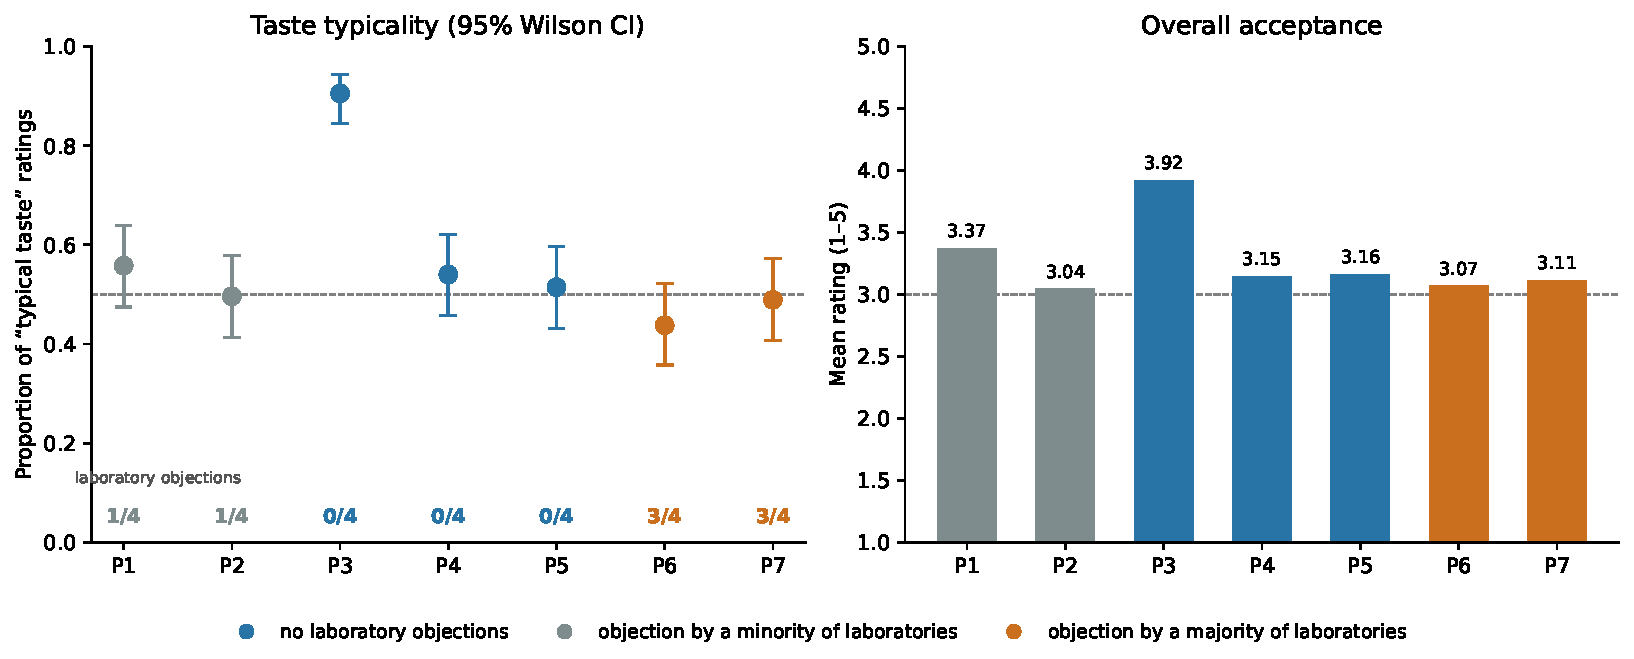
\includegraphics[width=16cm]{fig_panel_lab.pdf}
\end{adjustwidth}
\caption{Taste typicality (points, 95\% Wilson interval) and overall acceptance
(bars) of the seven samples in the blind consumer panel. Color indicates the
laboratory verdict: blue, no objections; grey, objection by a minority of
laboratories; orange, objection by a majority. Numbers at the bottom of the
left panel: number of laboratories (out of four) that rated the odor or taste
as not typical. Dashed lines: 0.5 and 3.\label{fig:panel_lab}}
\end{figure}

The samples flagged by the majority of laboratories (P6 and~P7) obtained
a typicality of 0.438 and 0.489 in the panel, lower than the mean
but indistinguishable from 0.5 ($p = 0.171$ and $p = 0.864$). In the
paired analysis, the typicality of the remaining samples
(P1, P2, P3, P4 and~P5: 0.603) was higher than that of the flagged samples
(0.464); the difference was $\Delta = 0.140$ (95\% CI:
0.071--0.208; $p < 0.001$; $d = 0.34$),
and for overall acceptance $\Delta = 0.24$ points
($p = 0.011$) (Figure~\ref{fig:contrast}). After excluding P3,
the difference in typicality fell to $\Delta = 0.064$ and was no
longer significant ($p = 0.109$).

\begin{figure}[H]
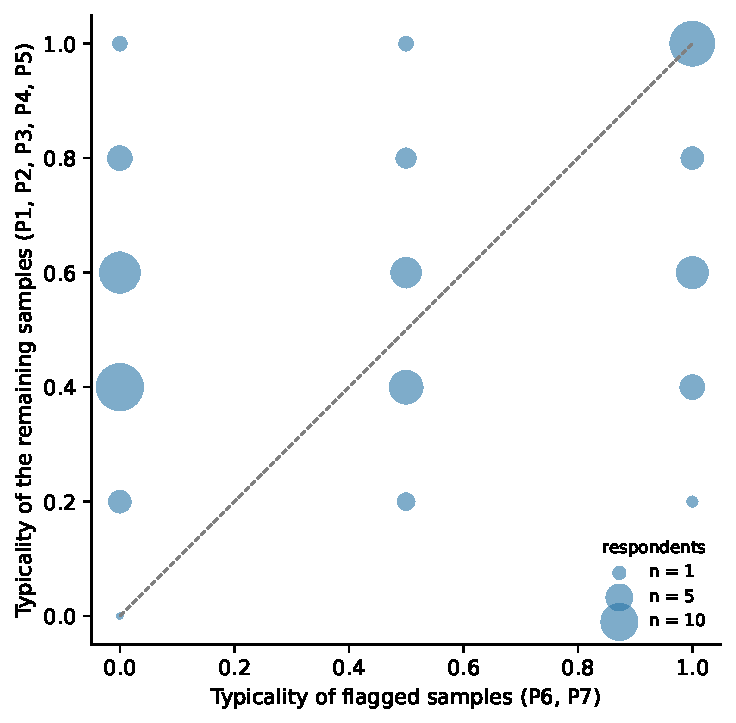
\includegraphics[width=8cm]{fig_contrast_lab.pdf}
\caption{Mean taste typicality of the samples to which the majority of
laboratories raised no objection ($y$-axis) and of the samples flagged by the
majority of laboratories ($x$-axis) for each respondent; point size: number of
respondents. Dashed line: equality of both ratings ($y = x$).\label{fig:contrast}}
\end{figure}

The panel did, however, register a feature consistent with some of the
laboratory descriptions: sweetness was rated as ``too strong'' most often for
P5 (41.3\%), P6 (40.9\%) and P7 (38.7\%), and least
often for P1 (22.1\%), P3 (22.6\%) and P2 (24.1\%).
Lab4 described the taste of P7 as ``very sweet'', which agrees with the panel
rating, but also the taste of P2, which the panel rarely rated as too sweet.


The blind consumer panel and the laboratories ranked the samples similarly in
terms of typicality, but they did not agree on which samples should be
considered not typical. The typicality ranking in the blind consumer panel
matches the laboratory ranking: sample~P3, to which the laboratories raised no
objections and which received the highest laboratory codes, was rated by far
the highest by consumers, whereas samples P6 and P7, flagged by three of the
four laboratories, were placed in the lower part of the ranking. Taste
assessment is therefore not devoid of content, since it reflects real
differences between honeys.

This agreement, however, rested on a single sample (P3), the only one
classified as typical by the blind consumer panel. After its exclusion, the
panel did not discriminate between the remaining six samples either in
typicality or in overall acceptance, and the typicality of P6 and P7 did not
differ significantly from 0.5: roughly half of the consumers considered the
taste of the samples flagged by most laboratories to be typical. The
difference between the flagged samples and the others was significant only
because of P3 and disappeared after its exclusion. The comparison on the same
scale shows this directly. The panel as a whole did not flag any sample, and
at the observed typicality a decision for P6 would require about
250~respondents. A single consumer agreed with a laboratory in 57.5\% of pairs
($\kappa = 0.10$), i.e., to a similar degree as with another consumer
($\kappa = 0.08$), whereas two laboratories agreed in 71.4\% of pairs
($\kappa = 0.30$). Typicality assessment thus recognizes clearly typical honey
but does not draw a sharp line between ``typical'' and ``not typical'' honey,
which is exactly the kind of line that a criterion of compliance with
commercial quality requirements needs.
